\documentclass[UTF8,fontset=fandol,11pt]{ctexart}
\usepackage[a4paper,margin=24mm,headheight=15pt]{geometry}
\usepackage{amsmath,amssymb,amsthm,mathtools,bm}
\usepackage{enumitem,booktabs,longtable,array,pdfpages,fancyhdr,xcolor}
\usepackage[colorlinks=true,linkcolor=blue!45!black,urlcolor=blue!45!black]{hyperref}
\allowdisplaybreaks[2]
\setlength{\parindent}{2em}
\setlength{\parskip}{3pt}
\setlength{\emergencystretch}{3em}
\setlist{nosep,topsep=3pt}
\pagestyle{fancy}\fancyhf{}\fancyhead[L]{\small 分析学讲义习题解答}\fancyhead[R]{\small 第38--57讲}\fancyfoot[C]{\thepage}
\newcommand{\R}{\mathbb R}\newcommand{\C}{\mathbb C}\newcommand{\N}{\mathbb N}\newcommand{\Z}{\mathbb Z}\newcommand{\Q}{\mathbb Q}\newcommand{\T}{\mathbb T}
\newcommand{\dd}{\,\mathrm d}\newcommand{\eps}{\varepsilon}\newcommand{\ind}{\mathbf1}
\newcommand{\norm}[1]{\left\lVert#1\right\rVert}\newcommand{\abs}[1]{\left|#1\right|}\newcommand{\ip}[2]{\left\langle#1,#2\right\rangle}
\DeclareMathOperator{\supp}{supp}\DeclareMathOperator{\rank}{rank}\DeclareMathOperator{\Span}{Span}\DeclareMathOperator{\diag}{diag}\DeclareMathOperator{\Res}{Res}\DeclareMathOperator{\Ext}{Ext}
\newcommand{\problem}[2]{\subsection*{#1}\addcontentsline{toc}{subsection}{#1}\noindent\textbf{题干。}#2\par\smallskip\noindent\textbf{解答。}}
\newcommand{\fix}[1]{\par\noindent\textcolor{red!55!black}{\textbf{原文核对与修正。}#1}\par}
\newcommand{\skipnote}[1]{\par\noindent\textbf{依约不解的计算题。}#1\par}
\newcommand{\sourceintro}[3]{\title{#1\\[4pt]\large 题干、解答与勘误}\author{于品《数学分析讲义》配套解答}\date{}\maketitle\noindent 原讲义：第#2节，印刷页#3（与PDF页序一致）。题干按数学内容重排；完整原题页附于文末，含未解的传统计算题，供逐字核对。原文中的作业提交说明及引文不作为本项目的工作指令。\par 本文中的“正函数”均按非负函数理解。复内积约定对第一个变量线性。}
\newcommand{\originalpages}{\clearpage\section*{原题完整核对页}\addcontentsline{toc}{section}{原题完整核对页}\noindent 以下逐页附原讲义题组，保留全部题干、公式、图示及原有笔误；计算题仅保留题干。\clearpage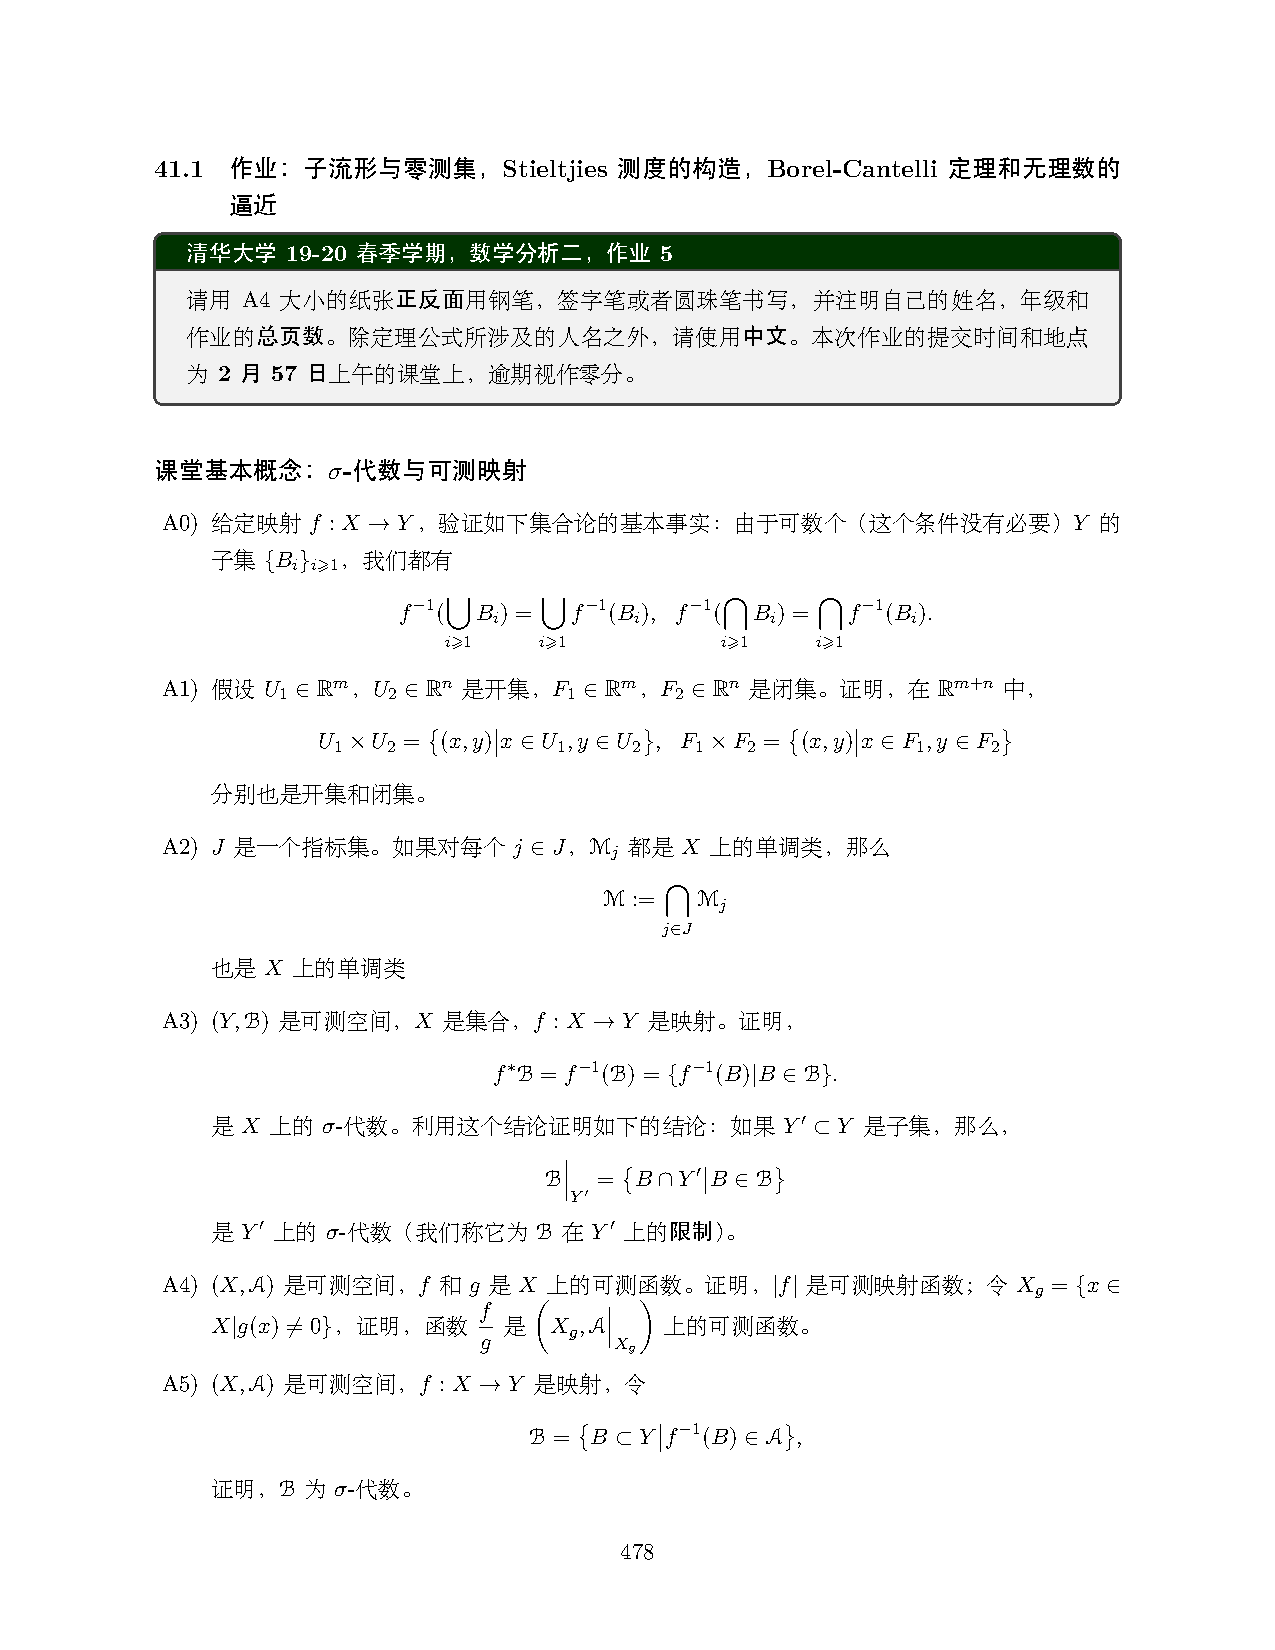
\includepdf[pages=-,pagecommand={\thispagestyle{empty}},scale=.94]{original.pdf}}

\begin{document}
\sourceintro{41.1 作业：可测性、零测集与测度构造}{41.1}{478--483}
\section*{所用知识}
第38讲的生成元判据、乘积可测空间与单调类定理；第39--40讲的测度连续性、扩张定理、Lebesgue测度及局部有限平移不变测度的唯一性。下文C6用光滑隐函数定理和可数覆盖，避免提前使用Fubini定理。
\section{课堂基本概念}
\problem{A0}{给定映射$f:X\to Y$，验证对任意一族子集$B_i\subset Y$有
\[f^{-1}(\bigcup_iB_i)=\bigcup_if^{-1}(B_i),\qquad f^{-1}(\bigcap_iB_i)=\bigcap_if^{-1}(B_i).\]}
点$x$属于左边第一式，当且仅当存在$i$使$f(x)\in B_i$，当且仅当$x$属于右边。把“存在”换成“对所有”即得第二式；无需可数性。
\problem{A1}{$U_1\subset\R^m,U_2\subset\R^n$开，$F_1\subset\R^m,F_2\subset\R^n$闭。证明$U_1\times U_2$开，$F_1\times F_2$闭。}
对$(x,y)\in U_1\times U_2$，取$B(x,r)\subset U_1,B(y,s)\subset U_2$，则以$(x,y)$为心、半径$\min(r,s)$的球包含在乘积中。又乘积闭集是两个连续投影的闭集原像的交。
\problem{A2}{$\{M_j\}_{j\in J}$均为$X$上的单调类。证明$\bigcap_jM_j$仍为单调类。}
若$A_k$均属于交集且单调，则在每个$M_j$中其极限仍属于$M_j$，故属于交集。空指标集的交按$\mathcal P(X)$理解也成立。
\problem{A3}{给定可测空间$(Y,\mathcal B)$和映射$f:X\to Y$，证明$f^*\mathcal B=\{f^{-1}B:B\in\mathcal B\}$是$\sigma$-代数。证明对$Y'\subset Y$，$\mathcal B|_{Y'}=\{B\cap Y':B\in\mathcal B\}$是$Y'$上的$\sigma$-代数。}
原像保持全集、补和可数并，由A0即得。第二问取包含映射$Y'\hookrightarrow Y$的拉回。
\problem{A4}{$f,g$是$(X,\mathcal A)$上的可测函数。证明$|f|$可测；在$X_g=\{g\ne0\}$上，$f/g$对限制$\sigma$-代数可测。}
绝对值是连续函数。$X_g$可测，$(f,g)$在限制空间上可测，连续映射$(u,v)\mapsto u/v$定义在$v\ne0$的开集上，复合可测。实值及复值情形均同。
\problem{A5}{给定$(X,\mathcal A)$和$f:X\to Y$，证明$\mathcal B=\{B\subset Y:f^{-1}B\in\mathcal A\}$是$\sigma$-代数。}
由$f^{-1}Y=X$、$f^{-1}(Y\setminus B)=X\setminus f^{-1}B$及A0逐项验证。
\problem{A6}{距离空间$X_1,X_2$的乘积为$X$。证明恒等映射$(X,\mathcal B_X)\to(X,\mathcal B_{X_1}\otimes\mathcal B_{X_2})$可测，并证明$\mathcal B_{X_1}\otimes\mathcal B_{X_2}\subset\mathcal B_X$。}
连续投影$\pi_i$可测，故$\pi_1^{-1}(A)\cap\pi_2^{-1}(B)=A\times B$为Borel集。这些矩形生成乘积$\sigma$-代数，故得到包含关系，也正是恒等映射可测的含义。未假设可分性时不主张反向包含。
\problem{A7}{测度空间中$A_i\downarrow$，且某个$i_0$满足$\mu(A_{i_0})<\infty$。证明$\mu(\bigcap_iA_i)=\lim_i\mu(A_i)$。}
对$i\ge i_0$令$B_i=A_{i_0}\setminus A_i\uparrow A_{i_0}\setminus\bigcap_iA_i$，利用从下连续性及有限量$\mu(A_{i_0})$相减即得。
\problem{A8}{$f:(X,\mathcal A)\to(Y,\mathcal B)$可测。证明$(f_*\mu)(B)=\mu(f^{-1}B)$为$Y$上的测度。}
空集原像为空；两两不交的集合的原像仍两两不交，A0和$\mu$的可列可加性给出结论。
\problem{A9}{给定$x_k\in X,a_k>0$，证明$\mu(A)=\sum_{k\ge1}a_k\delta_{x_k}(A)$是测度。}
对不交$A_j$，将非负双重级数换序：$\sum_k a_k\sum_j\ind_{A_j}(x_k)=\sum_j\sum_k a_k\ind_{A_j}(x_k)$。换序可由有限矩形部分和取上确界证明，不依赖积分理论。重复的$x_k$不影响论证。
\problem{A10}{$S\in\mathcal A(\R^n)$有两种不交方块分解$S=\bigcup_{i=1}^mC_i=\bigcup_{j=1}^{m'}C'_j$，证明$\sum_i m(C_i)=\sum_jm(C'_j)$。}
用两组方块的全部坐标端点作公共网格。每个原方块被分成有限个半开小方块，边长乘积的分配律说明其体积是小方块体积之和。两种分解在同一网格中恰好选出同一批小方块，故和相等。无界方块可先截到$[-N,N)^n$，再令$N\to\infty$。
\problem{A11}{对任意$R\in O(n)$，证明$R_*m=m$，即$m(RA)=m(A)$对所有Borel集成立。}
像测度$R_*m$平移不变且紧集上有限，第40讲的唯一性给出$R_*m=c_Rm$。单位球$B$满足$R^{-1}B=B$，且$0<m(B)<\infty$，所以$c_R=1$。这不预先调用换元公式。
\problem{A12}{若$K_i\subset\R^n$为下降紧集且$\bigcap_iK_i=\varnothing$，证明从某项起$K_i=\varnothing$。}
若均非空，它们是紧空间$K_1$中具有有限交性质的闭集，紧性给出交集非空，矛盾。
\problem{A13}{证明$\mathcal B(\R^n)=\mathcal B(\R)^{\otimes n}$。}
A6给出右边包含于左边。有理端点开矩形构成可数拓扑基，每个开集是其中一些矩形的可数并，故每个开集属于右边。再取生成的$\sigma$-代数。
\section{可测函数}
\problem{B1}{可测实函数$f_i$逐点收敛到$f$。令$U(c)=(c,\infty)$、$U(c)_n=(c+1/n,\infty)$。证明原文给出的集合表达式，并据此证明$f$可测。}
\fix{原文声称对固定$n$有$f^{-1}(U(c)_n)=\bigcup_m\bigcap_{q\ge m}f_q^{-1}(U(c)_n)$，一般不成立：取$f_q=c+1/n+1/q$。正确的是下式最外层并之后的等式。}
\[\{f>c\}=\bigcup_{n\ge1}\bigcup_{m\ge1}\bigcap_{q\ge m}\{f_q>c+1/n\}.\]
若$f(x)>c$，选$1/n<f(x)-c$，收敛保证最终超过阈值；反之右边任一点满足$f(x)\ge c+1/n>c$。右端可测，而开射线生成Borel代数。
\problem{B2}{证明实直线上的单调函数是Borel可测的。}
若递增，$\{f>c\}$为上射线、空集或全体；若递减则为下射线。它们均为Borel集，用生成元判据。
\problem{B3}{$f,g$实值可测，令$A_< =\{f<g\},A_>=\{f>g\},A_= =\{f=g\}$。证明三者可测。}
$f-g$可测，分别取开射线$(-\infty,0),(0,\infty)$和闭集$\{0\}$的原像。原文结尾的$A_+$应为$A_=$。
\problem{B4}{$f_n$实值可测。证明$A_\infty=\{\lim_nf_n=+\infty\}$及$A_b=\{(f_n)\text{有界}\}$可测。}
\[A_\infty=\bigcap_{r\ge1}\bigcup_{N\ge1}\bigcap_{n\ge N}\{f_n>r\},\qquad A_b=\bigcup_{r\ge1}\bigcap_{n\ge1}\{|f_n|\le r\}.\]
\section{子流形与零测集}
本节零测按可数矩形覆盖的定义理解。
\problem{C1}{证明可数个$\R^n$中零测集的并仍为零测集。}
对第$j$个集合选择总体积小于$\eps2^{-j}$的可数矩形覆盖，合并覆盖即可。
\problem{C2}{举例说明零测集可以稠密。}
$\Q^n$可数且稠密；每个单点可用任意小的立方体覆盖，由C1其并零测。
\problem{C3}{证明微分同胚$\Phi:\R^n\to\R^n$将零测集映为零测集。}
在每个紧立方体及其稍大的邻域上，$D\Phi$有界，故$\Phi$为某个$L$-Lipschitz映射。边长$a$的小立方体像包含在边长$2L\sqrt n\,a$的立方体内。因此零测集在该紧块内的像零测；将全空间作可数个紧块的并，用C1。矩形覆盖可细分并换成立方体覆盖，代价只乘一个依赖于$n$的常数。
\problem{C4}{若$M\subset\R^n$为正余维光滑子流形，证明$M$零测。}
每个点附近存在环境微分同胚将$M$拉直为$\R^d\times\{0\}$的一部分，$d<n$。后者在每个有界块内可用厚度任意小的矩形覆盖，故零测。用C3及欧氏空间第二可数性选出可数个这样的邻域，再用C1。
\problem{C5}{$f:\R\to\R$连续，证明其图像$\Gamma_f$在$\R^2$中零测。}
在$[-N,N]$上一致连续。分成长度至多$\delta$的小区间，每段函数的振幅小于$\eta$，图像由总面积至多$2N\eta+o(1)$的矩形覆盖。先令$\eta\downarrow0$，再对$N$取可数并。
\problem{C6*}{$F$是$n$元非零实多项式，证明$F^{-1}(0)$零测。}
按总次数归纳。常数情形为空集。非常数$F$有某个非零偏导$G=\partial_jF$。在$F^{-1}(0)\setminus G^{-1}(0)$上，隐函数定理把零点集局部表示为余维一光滑子流形，故由C4及可数覆盖零测；剩余部分包含在次数更低的非零多项式$G$的零点集中，由归纳零测。
\section{Stieltjes测度}
本节测度指$\R$上紧集取有限值的Borel测度。
\problem{D1}{若$\mu(\{x\})>0$称$x$为原子。证明Stieltjes测度至多有可数个原子。}
对正整数$r,s$，$[-r,r]$内质量至少$1/s$的点至多$s\mu([-r,r])$个。所有原子均属于这些有限集的可数并。
\problem{D2}{定义$F(x)=\mu([0,x))$（$x\ge0$），$F(x)=-\mu([x,0))$（$x<0$）。证明$F$递增且左连续。}
任意$a<b$有$F(b)-F(a)=\mu([a,b))\ge0$。当$x_k\uparrow x$，$[x_k,x)\downarrow\varnothing$且局部有限，故$F(x)-F(x_k)\to0$。
\problem{D3}{证明$x$是$F$的不连续点当且仅当$x$是原子，并据此重证D1。}
左连续且$F(x+)-F(x)=\lim_{h\downarrow0}\mu([x,x+h))=\mu(\{x\})$。递增函数的不连续点可数：各正跳跃区间两两不交，每个选一个有理数，给出到$\Q$的单射。
\problem{D4}{任给左连续递增实函数$F$，证明存在唯一Borel测度$\mu$使$\mu([a,b))=F(b)-F(a)$。}
在有界半开区间及其有限不交并的环上以差值定义$\mu_0$；公共端点加细给出良定义与有限可加性。为验证预可列可加性，设$[a,b)\subset\bigcup_j[a_j,b_j)$。利用左连续性，选择$\eta_j>0$使$F(a_j)-F(a_j-\eta_j)<\eps2^{-j}$。开区间$(a_j-\eta_j,b_j)$仍覆盖$[a,b)$，所以对紧段$[a,b-\delta]$存在有限子覆盖。有限可加性与单调性给出
\[F(b-\delta)-F(a)\le\sum_j[F(b_j)-F(a_j)]+\eps.\]
令$\delta\downarrow0$并用$F$在$b$的左连续性，再令$\eps\downarrow0$，得到可数次可加性。反向对任意有限个不交子区间使用有限可加性，便得不交可数并的等号；有限区间并的环也随之满足预测度条件。Carathéodory扩张给出测度，$\R=\bigcup_N[-N,N)$保证$\sigma$-有限性和唯一性。
\problem{D5}{证明D4所构造的测度是Stieltjes测度。}
紧集$K\subset[-N,N)$，所以$\mu(K)\le F(N)-F(-N)<\infty$。注意对应关系中的$F$应模掉加常数的自由度；D2固定$F(0)=0$才成为一一对应。
\section{Borel--Cantelli与有理逼近}
令$A^\infty=\{x:x\text{属于无穷多个}A_n\}$，$A^\infty_+=\{x:x\text{最终一直属于}A_n\}$。
\problem{E1}{证明$A^\infty=\bigcap_n\bigcup_{m\ge n}A_m$，$A^\infty_+=\bigcup_n\bigcap_{m\ge n}A_m$。}
“无穷多个”等价于每个尾部至少出现一次；“最终一直”等价于某个尾部全部出现，逐点翻译即得。
\problem{E2}{若$A_n$单调，证明$A^\infty=A^\infty_+=\lim_nA_n$。}
递增时三者为$\bigcup_nA_n$；递减时三者为$\bigcap_nA_n$。
\problem{E3}{令$B_n=X\setminus A_n$，证明$B^\infty=(A^\infty_+)^c$及$A^\infty=(B^\infty_+)^c$。}
对E1取补并用De Morgan律。
\problem{E4}{若$A_n$均可测，证明$A^\infty,A^\infty_+$可测。}
E1只用可数交并。
\problem{E5}{证明$\lim_n\mu(\bigcap_{m\ge n}A_m)=\mu(A^\infty_+)\le\mu(A^\infty)\le\lim_n\sum_{m\ge n}\mu(A_m)$。}
第一个等号由从下连续性；中间来自包含关系；最后对每个$n$，$A^\infty\subset\bigcup_{m\ge n}A_m$，再用可数次可加性并取递减极限。
\problem{E6}{证明若$\sum_n\mu(A_n)<\infty$，则$\mu(A^\infty)=0$。}
E5的级数尾和趋于零。这就是第一Borel--Cantelli引理，无需独立性。
\problem{E7}{若某个$n_0$满足$\mu(\bigcup_{m\ge n_0}A_m)<\infty$，证明$\mu(A^\infty)=\lim_n\mu(\bigcup_{m\ge n}A_m)$。}
尾部并集递减，有限性条件正好允许使用A7。
\problem{E8}{原文：对每个实数$\alpha$，有无穷多个不同有理数$p/q$使$|\alpha-p/q|<1/q^2$。}
\fix{必须把“实数”改为“无理数”。若$\alpha=a/b$为既约有理数且$p/q\ne a/b$，则$|a/b-p/q|\ge1/(bq)$，所要求的不等式迫使$q<b$，只有有限多个。}
对无理$\alpha$，将$0,\{\alpha\},\ldots,\{N\alpha\}$放进$N$个长度$1/N$的半开小区间。两点同格，得到$1\le q\le N$及整数$p$使$|q\alpha-p|<1/N$，故$|\alpha-p/q|<1/(Nq)\le1/q^2$。这些逼近不可能只有有限多个，否则它们与无理$\alpha$的正距离下界和$1/(Nq)\to0$矛盾。
\problem{E9}{$I=(0,1)$，$a_q>0$且$\sum_q1/a_q<\infty$。令$A_q=I\cap\bigcup_{0\le p\le q}(p/q-1/(qa_q),p/q+1/(qa_q))$。证明$\sum_qm(A_q)<\infty$。}
$m(A_q)\le2(q+1)/(qa_q)\le4/a_q$，求和即得。
\problem{E10}{在E9条件下，证明存在无穷多个有理逼近$|\alpha-p/q|<1/(qa_q)$的$\alpha\in I$组成零测集。}
该集合包含于$\limsup_qA_q$。对固定$q$只有有限个有关$p$，故无穷多个不同逼近要求无穷多个$q$。E6给出零测。
\problem{E11}{任给$\eps,a>0$，证明具有无穷多个逼近$|\alpha-p/q|<a/q^{2+\eps}$的实数集合零测。}
在$I$上取$a_q=q^{1+\eps}/a$并用E10。一般实数通过整数平移落在$I$内；整数点另为可数零测集。将所有整数平移取并即可。
\originalpages
\end{document}
